\documentclass[10pt,final]{article}
\usepackage{amsmath}
\usepackage{titlesec}
\usepackage{graphicx}
\usepackage{float}
\usepackage{wrapfig}
\usepackage{caption}
\usepackage{helvet}
\renewcommand{\familydefault}{\sfdefault}
\usepackage{subcaption}
\usepackage[color=cyan!40,obeyFinal]{todonotes}
\usepackage[margin=0.5in]{geometry}
\usepackage{cleveref}
\usepackage{microtype} %sexy kerning
\usepackage{color} % colors
\usepackage{ulem} % strikethrough
\usepackage{ifdraft}
\usepackage[	backend=biber,
		style=numeric-comp,
		sorting=none]{biblatex}
\addbibresource{ace.bib}

\date{}
\titleformat{\subsection}
  {\normalfont\fontsize{11}{17}\sffamily\bfseries\slshape}
  {\thesubsection}
  {1em}
  {}

\setcounter{secnumdepth}{4} % paragraph acts as subsubsubsection

\newcommand{\subsubsubsection}[1]{\paragraph*{#1}}

% only show strikethrough text when draft
\renewcommand{\xout}[1]{\ifdraft{\xout{#1}\fi}{}}
% toggle for displaying instructions
\newif\ifinstr
\instrtrue

%If true, display \instr wrapped text, but only if draft mode on
\newcommand{\instr}[1]{\ifdraft{\ifinstr {\color{cyan}\emph{#1}} \fi}{}}

%pKa formatting
\newcommand{\pKa}{$\mathrm{p}K_\mathrm{a}$\ }
\newcommand{\pH}{$\mathrm{pH}$\ }

\begin{document}
\listoftodos[Things that need to be done]\newpage
\section*{\centering Specific Aims}
Among the most fundamental molecular interactions in biology are those of small molecules with their macromolecular partners.
Endogenous small molecules play the role of messengers in many signaling pathways of the cell, and small molecule drugs interact with proteins in signaling cascades to modulate their function.
Understanding their interactions is vital to understanding many biological systems, and critical to drug development efforts.
Despite having catalogued many of the physical driving forces behind small molecule recognition, there are enormous gaps in our knowledge preventing us from articulating a quantitative, predictive understanding of small molecule affinities and selectivities for biomolecules.

In principle, \textbf{alchemical free energy calculations} provide a framework for quantitatively describing all aspects of the thermodynamics of small molecule recognition. However, deficiencies in our quantitative understanding of binding create large challenges in the ability of these calculations to reproduce experimental data in many systems, holding back their use in probing function and aiding design.
In this proposal, we address \textbf{three of the most significant open challenges in the quantitative modeling of small molecule recognition}.

\subsection*{Aim 1. Establish a correct quantitative treatment of alchemical free energy calculations for binding of charged ligands}
The soluble form of many drugs and endogenous small molecules is charged.
Yet, retrospective studies and predictive challenges show current free energy methodology fails for charged species\cite{Rocklin2013b,Muddana2014a}.
A number of corrections for calculations with charged ligand species have been proposed, but (1) consensus, and (2) a good model system to test and to confirm theory are lacking.
We propose using a computationally and experimentally tractable model system---the association of small-molecule guests with high-affinity supramolecular hosts---as a way to test, validate, and refine both theory and algorithms applicable to charged ligands.
The experimental datasets collected here will allow us to \textbf{ perform free energy calculations}, and to \textbf{ evaluate proposed corrections} in order to refine theory and algorithms as necessary.
We will utilize \textbf{ isothermal titration calorimetry (ITC) experiments}, which provide a “gold standard” biophysical assay for binding affinities.
We will additionally develop Bayesian approaches to accurately \textbf{ quantify measurement uncertainty} and allow for model-error propagation. 

\subsection*{Aim 2. Quantify the magnitude of protonation state effects on binding}
Proteins and many small-molecule drugs contain titratable moieties that can change protonation state upon binding or sample mixtures of protonation states, often in a conformation-dependent manner.
While detailed biophysical studies of a few specific model systems have demonstrated that these effects can contribute several kcal/mol in binding affinity, the true scope of the problem in ligand recognition in general is completely unknown.

We will use computational techniques to conduct a survey to assess the importance of protonation state issues in protein-small molecule interactions across a range of systems of pharmacological interest.
Existing \textbf{ \pKa prediction tools will be benchmarked against experimental small molecule \pKa data}, and then \textbf{ used for constant-\pH alchemical free energy calculations}.
We will perform complementary experiments on a tractable but disease-relevant system---kinase catalytic domains that can be expressed in E. coli---using \textbf{ fluorescence binding experiments } developed in our laboratory.

\subsection*{Aim 3. Develop a framework for alchemical free energy calculations to describe weak association and multiple binding}
Weak binding and association of multiple ligands are ubiquitous interactions in biological and pharmaceutically relevant systems.
In addition, drug discovery approaches such as fragment-based ligand design depend predominantly on a reliable method for integrating data from biophysical experiments with modeling for these situations.
We will \textbf{ extend the framework of alchemical free energy calculations}  to include the potential for \textbf{ multiple (possibly weak) binding events } using a \textbf{ semi-grand canonical ensemble formalism}.

As a model system, we will use the pharmacologically relevant protein \textbf{ human serum albumin } (HSA), known to bind many small molecules (sometimes multiple species at a time) to a variety of distinct binding sites.
We will  \textbf{ overcome deficiencies in theory } by both developing new Bayesian ITC experimental analysis techniques to select among theoretical association models, as well as simulating ITC data directly from semi-grand canonical ensemble simulations.

\subsection*{} % Add some spacing

Completion of the work will provide modeling strategies for non-trivial challenges in protein-ligand association that currently have no working solution, as well as illustrate the scope of challenges that remain.

\section*{Research Strategy - Significance}
\instr{General background, significance in terms of basic science and disease relevance.}

\todo[inline]{How common are charged ligands? How does it affect calculations when we don't correct them?}
\todo[inline]{Humam serum albumin as an important ``off target''.}
\todo[inline]{Need to optimize fragment combinations in situ. Reduce screening costs?}
\todo[inline]{Amount of ligands that undergo protonation state changes}

\section*{Research Strategy - Innovation}
\instr{Explain how your proposal differs from what others have tried.}

\section*{Research Strategy - Approach}
\instr{Approach: More specific background information. Describe in detail the experimental design and research methods to be used. Technical hurdles to be overcome should be mentioned. Alternative approaches should be given for experiments that may not be feasible. Discussion of expected or possible results and their interpretation. Best format for each specific aim: a) rationale, b) methods, c) expected results, d) alternatives. Theory aims should follow a similar structure where possible.}

\todo[inline]{Explain Bayesian statistics (what detail?)}
\todo[inline]{Define some generic Bayesian models for ITC}


\subsection*{Aim 1. Establish a correct quantitative treatment of alchemical free energy calculations for binding of charged ligands}
\subsubsection*{Rationale}
The soluble form of many drugs and endogenous small molecules is charged. Yet, retrospective studies and predictive challenges show current free energy methodology fails for charged species\cite{Rocklin2013b,Muddana2014a}.
A number of corrections for calculations with charged ligand species have been proposed, but (1) consensus, and (2) a good model system to test and to confirm theory are lacking\cite{Reif2013a,Rocklin2013a}. We will perform experiments using a Bayesian methodology to obtain a robust dataset. We will then \textbf{ perform alchemical free energy calculations to compare proposed corrections}.
%\subsubsection*{Methods}
\subsubsubsection{Subaim 1.1: Develop a Bayesian analysis framework for isothermal titration calorimetry to allow for uncertainty estimation}
In order to test theoretical approaches such as free energy calculations, a robust experimental dataset is necessary to distinguish between fundamental issues with the model or experimental errors. 
We will develop Bayesian approaches to \textbf{accurately quantify measurement uncertainty and allow for model-error propagation}. 
\todo[inline]{Explain how to describe an ITC experiment in a Bayesian way, focussing on things like concentration uncertainty}
The simplest model of an ITC experiment of a ligand $\mathrm{X}$ binding to a macromolecule $\mathrm{M}$ consist of a series of $n$ injections, resulting in injection heats $q_n$,
\begin{align}
	q_n = V_\mathrm{cell} \Delta H \left( [\mathrm{MX}]_n - [\mathrm{MX}]_{n-1} \right) + \Delta H_0 \label{equation:liberated-heat}
\end{align}
where $V_\mathrm{cell}$ is the volume of the sample cell, $\Delta H$ is the enthalpy of binding, $[\mathrm{MX}]_n$ is the complex concentration after $n$ injections, and $\Delta_H0$ is an offset that captures effects such as dilution and mechanical heats of stirring.
\begin{figure}
	\centering
	\missingfigure[figcolor=yellow!40, figwidth=0.8\textwidth]{figure from abrf-mirg paper, show that concentration uncertainty is a major source of error}
	\caption{The experiments performed in the ABRF-MIRG'2 study reveal systematic underestimation of errors, due to not quantifying concentration uncertainty \cite{Myszka2003a}.}
\end{figure}
Errors in the concentration of prepared solutions are a major source of uncertainty in ITC data. Not taking these into account can lead to orders of magnitude underestimation of the uncertainty of the experiments \cite{Myszka2003a}. One way to take this into account is by doing repeat experiments instead of technical replicates \cite{Vaux2012a}. This however is more time and material consuming, and therefore not a popular option among most scientific authors. 

To get the most out of single experiments, we can perform inference by applying a Bayesian approach. The concentration uncertainty can be modeled using a prior probability distribution around the expected concentration. Using Markov Chain Monte Carlo (MCMC) \cite{Metropolis1953a,Hastings1970a}, we can then sample from a posterior probability distribution to estimate the actual concentration,

\[
\mathcal{P} \left(\Delta G_\mathrm{bind}, \Delta H_\mathrm{bind}, \Delta H_0, [\mathrm{X_{syr}}], [\mathrm{M_{cell}}], \sigma \biggl{|} \prod\limits_{m=1}^{M}\{q_m\}^{N}\right) \quad,
\]
, where $\Delta G_\mathrm{bind}$ is the binding affinity, $\Delta H_\mathrm{bind}$ is the binding enthalpty, $\Delta H_0$ is the mechanical heat of injection and dilution, $[\mathrm{X_{syr}}]$ is the true syringe concentration, $[\mathrm{M_{cell}}]$ is the true cell concentration, and $\sigma$ is the measurement noise.

\todo[inline,color=green!40]{explain how we prevent overfitting by using Bayesian methods}


The methodology will allow incorporation of multiple experiments, such as calibrations, to accurately separate out heat effects due to e.g. dilution of the chemicals used or mechanical effects of the injections.
\begin{align}
	 \mathcal{P}\left(\Delta G_\mathrm{bind}, \Delta H_\mathrm{bind}, \Delta H_\mathrm{dil},\Delta H_\mathrm{mech}, [\mathrm{X_{syr}}], [\mathrm{M_{cell}}], \sigma \biggl{|} \prod\limits_{m=1}^{M}\{q_m\}^{N}\right) \quad,
\end{align}
for $N$ injections per $M$ experiments. Calibration experiments can provide more certainty by separating out parts of the effects, such as dilution.
\todo[inline]{Explain that we can incorporate multiple experiments}

\todo[inline,color=orange!40]{kriging/gaussian process baseline to deal with baseline drift. no dragging around datapoints as in origin etc, also refer to nitpic way of doing things?}
Furthermore, we will construct baseline models using gaussian process regression with scikit-learn\cite{Pedregosa2011a}.
\todo[inline,color=red!40]{skip experimental design?}

\xout{We can apply high dynamic range type experiments to perform trial experiments that allow us to find the order of magnitude of the affinity.
This estimate can then be used for experimental design, determining the optimum conditions for our experimental setup.
We will simulate the outcome of ITC experiments using MCMC and then perform them to validate the results.}

\todo[inline, color=black!40]{insert preliminary data figure as illustration of the type of data that we will be generating?}

\subsubsubsection{Subaim 1.2 : Obtain isothermal titration calorimetry data with quantified uncertainty for host-guest systems}

We will utilize ITC experiments, which provide a “gold standard” biophysical assay for binding affinities.
We propose using the association of small-molecule guests with high-affinity supramolecular hosts as a way to test, validate, and refine both theory and algorithms applicable to charged ligands.
We will use cucurbit-7-uril \cite{Lagona2005a} as a host, which is known to bind a series of cations within a range of affinities spanning several orders of magnitude \cite{Cao2013a}.
\todo[inline, color=red!40]{Move this part to the general rationale, using host-guest as a given for all subaims}

\subsubsubsection{Subaim 1.3: Perform a quantitative comparison of suggested correction models to experiments to establish a correct treatment of charged ligands in alchemical free energy calculations}
We will compare several methods that correct for changes in net charge of the system in alchemical free energy calculations\cite{Reif2013a,Rocklin2013a}.

\todo[inline,color=green!40]{Explain the theory behind the two methods short, equations, show how they are different}
\missingfigure[figcolor=cyan!40, figwidth=0.8\textwidth]{Some illustation of alchemically removing salt pairs would be nice}

Additionally, we will simulate by eliminating salt pairs, keeping the net charge of the system constant and assert the necessity of corrections to the free energy calculation.

\subsubsection*{Expected results}
Estimates of the experimental uncertainty will allow us to distinguish model errors from variance in the experimental data.
The work will enable the comparison of the proposed charge correction models. It is possible that all methods produce comparable results, in which case we will
The key question will then be whether any of the corrections  match up to experiment.
We will then be able to recommend a methodology to use when calculating the free energy of binding for charged species, enabling reliable simulations that are impossible to perform otherwise.
\subsubsection*{Pitfalls and alternatives}
\todo[inline,color=red!40]{What to do if the experimental uncertainty remains too high?}
\todo[inline,color=red!40]{What if none of the models agree with experiment?}
\todo[inline,color=red!40]{How do we pick a model if they all seem to agree? Can they all be correct?}

Issues with the molecular dynamics force field can influence the outcome of free energy methods in unpredictable ways. If the force field proves to be a troublesome factor, we will attempt to reparametrize our molecules to improve agreement with experiments.

\subsection*{Aim 2. Quantify the magnitude of protonation state effects on binding}
\subsubsection*{Rationale}
Proteins and many small-molecule drugs contain titratable moieties that can change protonation state upon binding or sample mixtures of protonation states, often in a conformation-dependent manner.
\missingfigure[figcolor=orange!40, figwidth=0.8\textwidth]{imatinib protonation states}
While detailed biophysical studies of a few specific model systems have demonstrated that these effects can contribute several kcal/mol in binding affinity\cite{Aleksandrov2007a,Czodrowski2007a,Neeb2014a}, the true scope of the problem in ligand recognition in general is completely unknown.
\todo[inline,color=cyan!40]{explain Czodrowski example}
\textbf{The usual approach in modeling ignores these problems and assumes a single protonation state} for an entire system. Our aim is to \textbf{rectify this by using constant-\pH simulations} in the context of alchemical free energy calculations. Using computational \pKa prediction techniques to provide input for this framework will enable future consideration of these effects.

\xout{We will use computational techniques to conduct a large scale survey to broadly assess the importance of protonation state issues in protein-small molecule interactions across a range of systems of pharmacological interest.}
\todo[inline,color=yellow!40]{develop techniques to deal with the protonation state issues}
\xout{Existing \pKa prediction tools will be benchmarked against small molecule \pKa data, and then used together with Monte Carlo titration codes (both extant and developed for this project) to provide an estimate of the scope of the problem.}
\todo[inline,color=purple!40]{short explanation constant-\pH simulations}

% \subsubsection*{Methods}
\subsubsubsection{Subaim 2.1: Obtain reliable small molecule \pKa predictions for kinase inhibitors}
Our aim is to \textbf{quantify the contribution of protonation state changes to binding} interactions. Experimental \pKa data is not widely available, so in part we will need to rely on computational \pKa prediction tools. We will \textbf{benchmark existing \pKa prediction tools}  using \pKa data obtained for a series of \textbf{kinase inhibitors} using a Sirius T3 instrument. This will provide a means to select a tool that can adequately predict \pKa values for kinase inhibitors with similar chemical components.

Preliminary results suggest that \textbf{several kinase inhibitors have access to multiple states  at physiological \pH}. For instance, the intracellular \pH of most tumors is around 7.2 \cite{Griffiths1991a,Stubbs2000a}. Preliminary data in \Cref{figure:pka-kinase} indicates that a number of FDA approved kinase inhibitors have \pKa values close to the physiological \pH.
\begin{figure}[H]
	\centering
	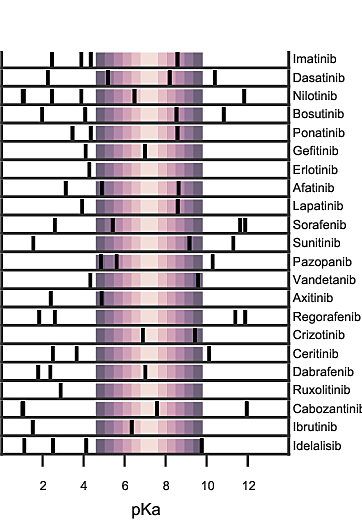
\includegraphics[width=0.27\textwidth]{figures/inhibitor-pKas.png}
	\caption{Protonation states accessible to FDA approved kinase inhibitors. Colors indicate accesibility of states at \pH 7.2 within blocks of $k_BT$ units of energy, where darker means more units of $k_BT$ away from the accesible region. Preliminary data obtained using Epik.\cite{Shelley2007a,Greenwood2010a}}
	\label{figure:pka-kinase}
\end{figure}

\todo[inline,color=blue!40]{summary of available \pKa prediction tools.}
Among the tools considered will be \textbf{MoKa}\cite{Milletti2007a}, \textbf{Jaguar}\cite{Bochevarov2013a}, and \textbf{Epik}\cite{Shelley2007a,Greenwood2010a}.
MoKa generates \pKa's based on atomistic descriptors, defined by the surrounding atoms. The descriptors are based on molecular interaction fields calculated using GRID \cite{Goodford1985a} for a library of 3D fragments, but can succesfully be applied on 2D structures.
Schrodinger's Jaguar provides means of estimating \pKa values using quantum mechanical methods.
Epik uses Hammett Taft linear free energy approaches\cite{Perrin1981a} for predicting \pKa values .

\subsubsubsection{Subaim 2.2: Idenification of kinase-ibhibitor combinations with potential protonation features}
To accurately incorporate \pKa effects into our simulations, we also need to consider that the \pKa of protein residues may change on binding of a ligand. 

Using kinases as model systems, we will survery small molecule-kinase interactions using MCCE\cite{Song2009a}, which will be extended to incorporate small molecules in its calculations.
We will make a selection of crystal structures from the protein data bank (PDB)\cite{Berman2000a} of kinases with inhibitors bound. 
We can then selecting for systems that show potential mixtures of protonation states at physiological \pH values as indicated by their multiconformer \pKa prediction to use in constant-\pH simulation as part of our aim. 


\subsubsubsection{Subaim 2.3: Estimate the effect of protonation states on binding affinity through experiment and computation}
The obtained data from the \pKa survey will allow us to set up alchemical free energy calculations that employ semi-grand canonical contant-\pH methods.\cite{Mongan2004a}

The calculations will be performed using openMM\cite{Eastman2013a} and Yank \cite{Chodera2015a}. We will also perform simulations that do not apply the constant-\pH methods. This will allow us to estimate the effect of protonation state changes on the binding affinity.

We will \textbf{validate the results of the free energy calculations by performing complementary experiments} on kinase catalytic domains that can be expressed in E. coli using ITC experiments. \textbf{The change of protonation states can be observed in ITC by performing replicate experiments using buffers of different ionization energies}. This will lead to an enthalpic contribution/penalty to the binding affinity.

This data can then be compared to our simulations, to assertain whether they can recapitulate the protonation state effects observed in experiment.

\todo[inline,color=violet!40]{short explanation constant-\pH simulations}

\subsubsection*{Expected results}
We expect to observe changes in protonation states in some proteins, though the degree by which they are ubiquitous is unknown. We will observe whether allowing for a mixture of protonation states makes a difference in a class of proteins such as kinases. In the case that changes in protonation state make a significant contribution, we will now have the tools to include this in our modeling. If the contribution appears to make no difference, we will have ruled out the need to use more expensive theoretical methods and more experimental resources.

\subsubsection*{Pitfalls and alternatives}
Currently evidence only exists for a small number of systems \cite{Aleksandrov2007a,Czodrowski2007a}. It is possible that the heat effect from changing protonation states, as observed in IT, is masked by larger heat effects that are part of the binding affinity. Alternative experiments could be performed using fluorescent kinase inhibitors that change their fluorescence signal when switching between protonation states.
By studying the available kinase-ligand complexes in the PDB we hope to have a representative selection of protein-ligand interactions, though potentially these contributions are different for other parts of the proteome. If the result is insignificant, we can attempt to extend our search to other classes of proteins, to rule out that protonation state changes significantly contribute to other proteins.

\subsection*{Aim 3. Develop a framework for alchemical free energy calculations to describe weak association and multiple binding}
\subsubsection*{Rationale}
Weak binding and association of multiple ligands are ubiquitous interactions in biological and pharmaceutically relevant systems.
In addition, drug discovery approaches such as fragment-based ligand design depend predominantly on a reliable method for integrating data from biophysical experiments with modeling for these situations. Characteristics such as stoichiometry are unknown and need to be modelled experimentally.
\todo[inline,color=blue!40]{what does origin already support? check their manual}
\todo[inline,color=green!40]{our goal is to build a quantitative connection}
As a model system, we will use the pharmacologically relevant protein human serum albumin (HSA), known to bind many small molecules (sometimes multiple species at a time) to a variety of distinct binding sites.
We will \textbf{overcome deficiencies in theory} by both developing new \textbf{Bayesian ITC experimental analysis techniques} to select among theoretical association models, as well as simulating ITC data directly from \textbf{semi-grand canonical ensemble simulations}.


\begin{center}
\missingfigure[figcolor=red!40,figwidth=0.8\textwidth]{structure of HSA}
\end{center}
% \subsubsection*{Methods}

\subsubsubsection{Subaim 3.1: Extend semi-grand canonical ensemble alchemical free energy calculation tools}
At current time, a framework to perform semi-grand canonical ensemble simulations with multiple ligands does not exist. Therefore we will extend the framework of alchemical free energy calculations to include the potential for multiple (possibly weak) binding events using a semi-grand canonical ensemble formalism. 
The total number of ligands bound to a target is governed by its chemical potential, $\mu$. Alchemical methods will allow us to insert new copies of ligands into our simulation without driving the system far away from equilibrium. 

\todo[inline]{Using NCMC?, Does this take care of larger ligands?, Implicit v Explicit solvent}	
\begin{center}
\missingfigure[figcolor=cyan!40, figwidth=0.8\textwidth]{alchemical semi-grand canonical example figure}
\end{center}

\subsubsubsection{Subaim 3.2: Validate computational predictions by applying Bayesian model selection on ITC  experiments}
To provide validation of our computational results, we will perform ITC experiments on HSA. Binding stoichiometry is not known a priori, yet if we want to deconvolute characteristics such as binding affinities for different sites, we need to model multiple binding sites with multiple affinities.
Origin, a conventional ITC analysis software package uses cooperativity parameters $n_i$ to describe multiple binding sites\cite{MicroCal2004a}.

\todo[inline,color=teal!40]{SEDPHAT?}

To solve this problem, we will extend our Bayesian analysis tools with the capacity to use Bayes factors to select between possible models \todo[inline]{Is this the method most suited?}
Individual binding associations can be modeled as
\todo[inline,color=red!40]{formulate a model that allows for multiple different associations, affinities etc}

\subsubsection*{Expected results}
Our Bayesian methodology will enable us to predict binding affinities to proteins with multiple binding sites. We will be able to deconvolute the effects of multiple species, as well as multiple binding sites. At the same time, we can now model these interactions computationally. This allows us to study the predicted interactions at an atomistic scale, as well as propose new experiments for interesting fragment or drug combinations, for instance multiple drugs binding to HSA at the same time).

\subsubsection*{Pitfalls and alternatives}
\todo[inline,color=red!40]{Possibility of not being able to deconvolute multiple binding sites, do adaptive experiments?}

\section*{Conclusion}
We have solved science.

% refs
\printbibliography

\end{document}
